\documentclass[11pt,a4paper]{article}

\usepackage[utf8]{inputenc}
\usepackage[T1]{fontenc}
\usepackage{lmodern}
\usepackage[margin=2.5cm]{geometry}
\usepackage{graphicx}
\usepackage{booktabs}
\usepackage{tabularx}
\usepackage{array}
\usepackage[font=small]{caption}
\usepackage{url}
\usepackage[hidelinks]{hyperref}

\renewcommand{\arraystretch}{1.15}
\newcolumntype{L}{>{\raggedright\arraybackslash}X}
\setlength{\parskip}{0.5em}
\setlength{\parindent}{0pt}
\graphicspath{{figures/}}
\renewcommand{\topfraction}{0.9}
\renewcommand{\bottomfraction}{0.8}
\renewcommand{\textfraction}{0.1}
\renewcommand{\floatpagefraction}{0.8}
\setcounter{totalnumber}{4}

\begin{document}

\begin{center}
{\Large Can AI-written data-quality rules be trusted?}\\[0.4em]
{\large MSc thesis proposal and pilot results}\\[0.8em]
Tomash Oosterbaan\\
MSc Artificial Intelligence, University of Groningen\\
Graduation project context: Avanade and Rabobank\\
October 2026
\end{center}

\section{The problem}

Banks use data from many sources, and data from a new source is rarely ready for use. Before it reaches reports, models or decisions, a data team checks it with validation rules: required fields must be present, values must have the right type, codes must come from an agreed list, and known business rules must hold. Long Tran described this kind of work in his context at Rabobank: technical validation, business rules, monitoring thresholds, pass and fail checks, and manual investigation of exceptions \cite{tran}. A public Rabobank case study also mentions missing data and differences between information providers as practical problems \cite{alderse}. These observations motivate the example below; they are not a description of Rabobank systems, and no Rabobank data is used.

Writing good rules takes time and domain knowledge. Language models, the kind of AI behind tools like ChatGPT, can now write such rules in seconds, and data-quality tools are starting to offer this \cite{rehberger}. The problem is that a team cannot easily tell whether an AI-written rule is right. Suppose a credit team wants to use the financial statements that its business clients publish. An analyst asks a model for checks and gets twenty rules back, such as ``total assets must equal liabilities plus equity''. Some are useful. Others look reasonable but flag hundreds of correct numbers per company, or miss the errors they were meant to find. Asked again the next day, the model may write a different rule. A wrong rule is not harmless: it lets errors through or floods the team with false alarms, and every alert costs an employee's time. A rule that nobody can explain is also hard to defend to an auditor.

\section{The idea}

We want to test AI-written rules the way you would test the work of a new colleague: against the work of experts, on cases where the answer is known, and more than once. The idea has three parts.

First, an expert reference. We use public data-quality rules that a committee of experts wrote, together with their official test cases (Section~\ref{sec:data}). If a model writes its own version of such a rule, we can check whether it finds the same problems.

Second, a stress test. We put known errors into real data and see which ones each control catches: the expert rules, simple statistical checks, and AI-written rules. This shows what the existing controls miss and whether AI rules fill that gap. Simple statistical checks are included everywhere, because AI is only worth its cost if it does better than a cheap method.

Third, a gate. An AI rule is only adopted after it passes criteria fixed in advance (it catches enough, gives few false alarms and gives the same result when generated again) and after a person approves it.

The working research question is:

\begin{quote}
To what extent can LLM-generated validation rules provide reliable and reproducible error detection beyond expert-defined data quality controls in financial filings?
\end{quote}

We split it into five questions, because each needs a different reference (Table~\ref{tab:e}). A rule can copy an expert rule well and still add nothing, or catch many errors and still be useless because of its false alarms.

\begin{table}[htbp]
\centering
\small
\begin{tabularx}{\textwidth}{@{}p{0.7cm}LL@{}}
\toprule
 & Question & How we know the answer \\
\midrule
E1 & Can the AI reproduce an expert rule from its written description? & Official test cases of that rule \\
E2 & Which errors does each control catch? & Errors we put in ourselves \\
E3 & Does a control flag numbers that companies later corrected? & Corrections in amended reports (not proven errors) \\
E4 & What does AI add beyond expert rules and statistical checks? & Injected errors that the existing controls miss \\
E5 & Is the result stable, and how many alerts does it cost? & Repeated generations; alerts on reports that were never corrected \\
\bottomrule
\end{tabularx}
\caption{The five sub-questions.}
\label{tab:e}
\end{table}

This direction grew out of an earlier idea, which we also tested in a pilot: whether advanced error detectors, models that flag suspicious values directly instead of writing rules, add value beyond existing checks. Section~\ref{sec:pilot1} summarises that pilot and why we moved on.

\section{What earlier research says}

Detecting data errors is an old problem. Abedjan et al.\ ran several detection tools on real datasets and found that no single tool came close to finding all errors; combining tools found more, but each tool also added alerts that a person had to check \cite{abedjan}. Rule libraries such as Deequ make checks easy to define and can suggest simple rules from a profile of the data \cite{deequ}. Learned detectors flag values that do not fit patterns or relationships in the data \cite{cdc,raha,zeroed,autotest}. Jung et al.\ show that how errors are placed in the data changes which method looks best \cite{taberr}.

Several recent studies let language models write data-quality rules. LeDQeR generates rules from erroneous records and filters out rules that misfire on clean data \cite{ledqer}. Akella et al.\ let a model write Python checks with retrieval and guardrails \cite{akella}. AuDQ lets AI agents discover rules for banking and retail data, which people then rate; the authors note that neither dataset ``ships with a reference rule set to compare against'' \cite{audq}. Alexander et al.\ compared tests written by GPT-3.5 and GPT-4 with a suite written by one experienced data scientist, and ran every setting five times to measure consistency \cite{alexander}. Two warnings come from related work: automatically discovered constraints are mostly false, ``rarely below 95\%'' for current algorithms \cite{martin}, and language models give different code across runs, even with settings meant to make them deterministic \cite{ouyang}.

Testing checks by injecting errors is also known. Homayouni et al.\ used it to test checks in data warehouses \cite{homayouni}, and JENGA used it to improve the data checks of a machine-learning pipeline \cite{jenga}. In software testing, catching artificial faults is related to catching real faults \cite{just}. On financial filings, language models have mainly been used as judges that read a table and point at inconsistencies \cite{secfintables,finauditing}. Finally, people tend to trust automated suggestions too easily \cite{parasuraman}, and engineers describe too many alerts as a real problem in practice \cite{shankar}. This supports a gate with fixed criteria before a person decides.

\section{Data: what we use and why}
\label{sec:data}

The main data are financial filings, because they are public, real and financial, and because they come with an expert rule set. This section explains the three pieces simply.

Financial filings in XBRL. American listed companies send their annual and quarterly reports to the SEC. Besides the readable document, every number is also delivered in XBRL, a machine-readable format. Each number is a separate fact with a label from a standard dictionary, a period, a unit and a precision. For example: \texttt{Revenues} $=$ 5{,}000{,}000, from 1 January to 31 December 2024, in US dollars, rounded to thousands. Because every number has a fixed label and period, a computer can check it with rules. European listed companies use the same format for their annual reports (ESEF) \cite{esef}. Research shows that these filings contain real errors, for example signs entered the wrong way \cite{debreceny}.

The DQC rules. The Data Quality Committee (DQC) of XBRL US is a group of companies, data users and software firms. It publishes free rules that find common mistakes in these filings, about 200 so far \cite{dqc}. Companies and software vendors run them before a report is submitted. Table~\ref{tab:dqc} gives four examples. Each rule comes with three things: a written description of what it checks, the official implementation that runs in the open-source program Arelle \cite{arelle}, and official test cases. A test case is an example filing together with the exact messages the rule should give, like an answer key. Each rule also has a release date. This makes the DQC rules useful in three ways at once: they are an independent expert reference, they are the existing control a team would already have, and their test cases tell us whether an AI version of a rule finds the same problems.

\begin{table}[htbp]
\centering
\small
\begin{tabularx}{\textwidth}{@{}p{1.8cm}LL@{}}
\toprule
Rule & What it checks & Example message \\
\midrule
DQC\_0004 & Values that must be equal, such as assets and liabilities plus equity. & ``Assets with a value of 340,000,000 is not equal to the total of Liabilities and Equity with a value of 350,000,000.'' \\
DQC\_0009 & One value must not exceed another, such as shares outstanding and shares issued. & Shares outstanding is larger than shares issued. \\
DQC\_0014 & Amounts that should never be negative. & ``Derivative Assets has a value of -400,000 which is less than zero.'' \\
DQC\_0212 & If shares outstanding is reported, shares issued must be reported too. Released October 2025. & A value was reported for shares outstanding, but not for shares issued. \\
\bottomrule
\end{tabularx}
\caption{Four DQC rules in plain words. Quoted messages are from the rule documentation \cite{dqc}.}
\label{tab:dqc}
\end{table}

Corrections. When a company finds a mistake in a report, it can file an amended report. Comparing the original with the amendment shows which numbers changed. These are real corrections, but not necessarily data errors: many are accounting restatements. Brown et al.\ used such amendments as signals of misreporting \cite{brown}.

Table~\ref{tab:data} lists what we used in the pilots and what we plan to add. My supervisors suggested three to five datasets. Each planned dataset again comes with a public expert rule set, so the same design can be repeated. GLEIF and HMDA have a different structure from financial statements, which tests whether the results hold beyond one type of data.

\begin{table}[htbp]
\centering
\small
\begin{tabularx}{\textwidth}{@{}p{3.5cm}p{3.3cm}Lp{1.5cm}@{}}
\toprule
Data & Expert rules & Why & Status \\
\midrule
UCI Credit, Bank Marketing, Wine \cite{uci-credit,uci-bank,uci-wine} & none (our own rules) & Public tables for the first pilot; Credit is close to a bank credit file & Pilot 1 \\
SEC Financial Statement Data Sets \cite{fsds}, 2023 to mid-2025 & n/a & 68{,}875 filings; 1{,}294 original and amended pairs give real corrections & Pilot 2 \\
EDGAR XBRL filings & DQC US rules \cite{dqc} & 240 filings (120 never corrected, 120 later corrected) on which all controls run & Pilot 2 \\
ESEF annual reports of European companies \cite{esef} & DQC and XBRL International rules for IFRS and ESEF \cite{dqc} & Same format and rule engine, closest to Dutch practice & Planned \\
GLEIF legal entity records \cite{gleif} & GLEIF Data Quality Rule Setting & Reference data banks use to identify counterparties & Planned \\
HMDA mortgage data \cite{hmda} & Edits in the HMDA Filing Instructions Guide & Loan-level data; the public file is modified for privacy & Planned \\
FFIEC Call Reports & FFIEC validation edits & Bank balance sheets; machine-readable edits still to be checked & Optional \\
\bottomrule
\end{tabularx}
\caption{Data used in the pilots and planned for the thesis. All of it is public.}
\label{tab:data}
\end{table}

\section{Models: what we could use and why}

We only use open-weight models: models whose files can be downloaded and run on our own hardware. This has four advantages. No data leaves the organisation, which matters for a bank. There are no usage costs. The exact model file can be stored, so results can be reproduced. And the release date is known, so we can separate rules the model could have seen during training from rules it could not. Table~\ref{tab:models} shows the plan. Every AI result is compared with methods that use no AI.

\begin{table}[htbp]
\centering
\small
\begin{tabularx}{\textwidth}{@{}p{2.8cm}p{4.6cm}L@{}}
\toprule
Use & Models or methods & Why \\
\midrule
Pilot (done) & Qwen2.5-Coder-7B and Qwen3-8B \cite{qwen25coder,qwen3}, compressed to run on a normal processor & Free, local, one code model and one general model, known release dates \\
Main research & Larger versions of the same families (for example Qwen2.5-Coder-32B, Qwen3-32B) and a second family (gpt-oss-20b and 120b \cite{gptoss}) on the university GPU cluster & Tests whether model size and model family change the conclusions \\
Baselines without AI & Generic checks; statistical checks learned from other companies' filings; rule suggestion from data profiles as in Deequ \cite{deequ} & Shows whether AI does better than cheap methods \\
AI as judge & The same models, asked to point at suspicious numbers directly & Compares writing rules with judging data \\
Artefact & A small or medium model that runs on one machine, behind an adapter & A bank can plug in the model it has approved \\
\bottomrule
\end{tabularx}
\caption{Models and baselines.}
\label{tab:models}
\end{table}

\section{What could be new}

Much of this has been done before, and we will not claim it: AI-written data-quality rules \cite{ledqer,akella,audq}, comparison with one gold-standard suite and repeated runs \cite{alexander}, human approval of rules \cite{audq}, stress tests of checks with injected errors \cite{homayouni,jenga}, and language models as judges of financial tables \cite{secfintables,finauditing}.

What we did not find is the following. First, AI-written rules executed and compared with a large public rule set that experts wrote and approved independently of any study, using its official answer keys, and split by whether the rule was published before or after the model. Second, a measurement of what AI rules add beyond such an expert rule set and beyond statistical checks, with the number of false alarms next to it. Third, a map per error type of what official rule sets such as DQC, GLEIF and HMDA miss, and whether AI rules or statistics close that gap. The novelty would therefore be in the evaluation design and the reference, not in a new method. This is a narrow niche in a field that moves fast, so the literature will be checked again before any claim is made.

\section{What we did in the pilots}

\subsection{Pilot 1: do advanced detectors add value?}
\label{sec:pilot1}

The first pilot used three public UCI tables (Table~\ref{tab:data}), each with 800 evaluation records and separate historical records. We changed values in a copy and recorded which cells were changed: 630 scenarios with missing values, wrong types, invalid codes and scale changes, then 360 scenarios with changes that still pass the rules, such as a bill copied from the wrong month or a valid category replaced by another valid one. Changes were made in 1\%, 5\% or 10\% of values, placed at random, depending on another field, or depending on the value itself \cite{taberr}, with five repetitions.

The existing controls were rules, statistical checks learned from history, and simple prediction models (Ridge and logistic regression). On top of these we tested CDC \cite{cdc}, dBoost, LUCARIO \cite{lucario}, RIOLU \cite{riolu}, Auto-Test \cite{autotest}, Raha \cite{raha} and a small experiment inspired by ZeroED \cite{zeroed}. We assumed a reviewer can check 20 alerts per 800 records, and counted how many extra changed values a reviewer would actually see.

The rules caught every missing value, wrong type and invalid code. For changes that pass the rules, detectors did find extra changes, but buried in extra alerts (Figure~\ref{fig:a}). With 20 reviews, the net gain of CDC was $+0.4$ changed values for Bank, $0$ for Credit and $-1.0$ for Wine. After adding a simple logistic regression to the existing controls, the gain for Bank disappeared. On published benchmarks, Auto-Test added 5 and 4 correct findings at 25 reviews, 3 and 1 against a stronger pattern check, and 0 if existing alerts were reviewed first. Where a copy of the original source existed, simply comparing source and copy found every change.

\begin{figure}[htbp]
\centering
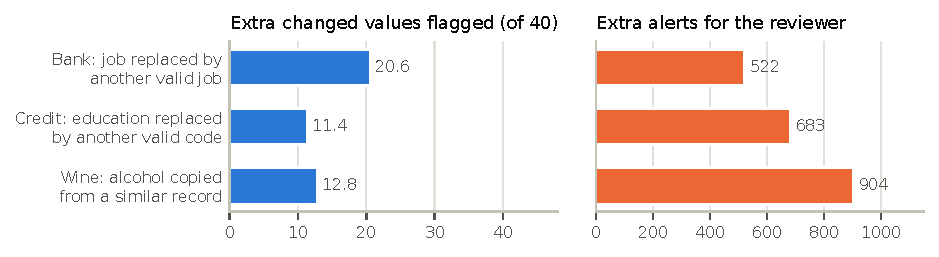
\includegraphics[width=\textwidth]{fig_a_increment.pdf}
\caption{Pilot 1. CDC added to rules, statistical checks and a Ridge model; 5\% changed values, mean of five runs. Left: changed values found that the existing controls missed. Right: extra alerts.}
\label{fig:a}
\end{figure}

The lesson was that strong cheap baselines and the number of alerts decide whether a detector is useful. But the idea itself was not new \cite{abedjan,rein}, all errors were made by us, and AI played only a small role. That is why we moved to AI-written rules with an expert reference.

\subsection{Pilot 2: AI-written rules on SEC filings}

We ran four kinds of existing controls on 240 filings: generic checks (for example the same number reported twice with different values), three statistical checks learned from 2023 and 2024 filings of other companies (unusual sign, unusual size, unusual jump between periods), a deliberately naive rule that amounts are never negative, and the official DQC rules in Arelle. We injected seven types of errors, one per copy of a filing, with placement and size based on the real corrections (Table~\ref{tab:ops}).

\begin{table}[htbp]
\centering
\small
\begin{tabularx}{\textwidth}{@{}p{3.2cm}L@{}}
\toprule
Injected error & Example \\
\midrule
Sign flipped & Net income of 120 becomes $-120$. \\
Value x1000 & 4{,}500 (in thousands) is entered as 4{,}500{,}000. \\
Amount changed & A value changes by a ratio seen in real corrections. \\
One digit changed & 18{,}340 becomes 18{,}390. \\
Wrong element & An amount is reported under a related but wrong label. \\
Periods swapped & This year's and last year's values are exchanged. \\
Fact removed & A reported number is missing. \\
\bottomrule
\end{tabularx}
\caption{The seven injected error types.}
\label{tab:ops}
\end{table}

The two models wrote rules as Python code in three ways: from the written description of a DQC rule (translate), from a sample of a filing (discover), and from a list of error types the existing controls missed on development filings (gap-closing). Rules that crashed got one repair round. All generated code ran in a sandbox, a separate process without network access. As a comparison, Qwen3-8B also acted as a judge that reads up to 120 facts of a filing and lists up to ten suspicious ones. AI rules were only evaluated on test filings no model had seen. Before running anything we fixed the gate: at most one alert per filing that was never corrected, at least 20\% of the missed errors caught, and the same result when run again.

Real corrections (E3). Of the 1{,}294 original and amended pairs, 631 changed at least one number, mostly through accounting restatements. In a check of 20 targeted corrections against the documents, the original number was wrong in 9 cases: 7 accounting restatements and 2 tagging errors (a wrong element and a wrong period length). In 3 cases it was not wrong, and in 8 it could not be determined. An AI model pre-filled these labels and I checked them against the SEC documents, so they are not an independent expert annotation. Two separate AI passes over the same items agreed on only 10 of 20, so corrections remain candidates. On later-corrected numbers, DQC flagged 1.6\% and the statistical checks 0.1 to 0.6\%. One AI rule set flagged 92.6\%, but only because it flagged almost everything.

Reproducing expert rules (E1) and stability (E5). Figure~\ref{fig:e1} shows the results. For rules published before the models, both found about 41\% of the official messages; for rules published after the models, 3\% and 13\%. Most rules scored 0\%, a few 97 to 100\%. A rule we translated by hand found 15 of 16 messages, so the test setup is not the cause. Writing the same rule three times often gave very different results, for Qwen3 from 0\% to 100\% on two of nine rules.

\begin{figure}[htbp]
\centering
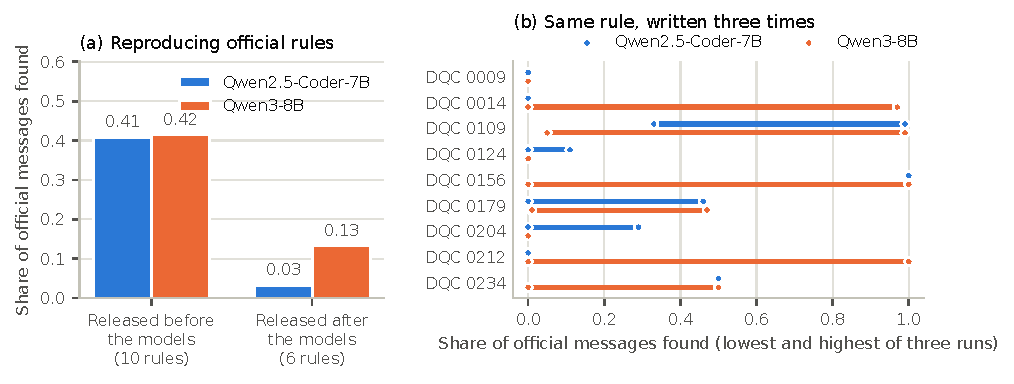
\includegraphics[width=\textwidth]{fig_b_e1_e5.pdf}
\caption{Pilot 2. (a) Share of official DQC messages found by rules the models wrote from the rule descriptions. (b) Lowest and highest result of three generations of the same rule.}
\label{fig:e1}
\end{figure}

Injected errors (E2). Figure~\ref{fig:catch} shows the catch rates on 12 test filings where all controls could be run. The three statistical checks together caught two thirds of the x1000 errors (82\% on all 66 test filings) and almost nothing else. DQC caught 64\% of swapped periods and 50\% of x1000 errors, but only 17 to 25\% of the other types and no removed facts. All existing controls together caught 27 of the 83 injected errors. The best AI rule set caught sign errors about as well as the naive ``never negative'' rule, and for the same reason.

\begin{figure}[htbp]
\centering
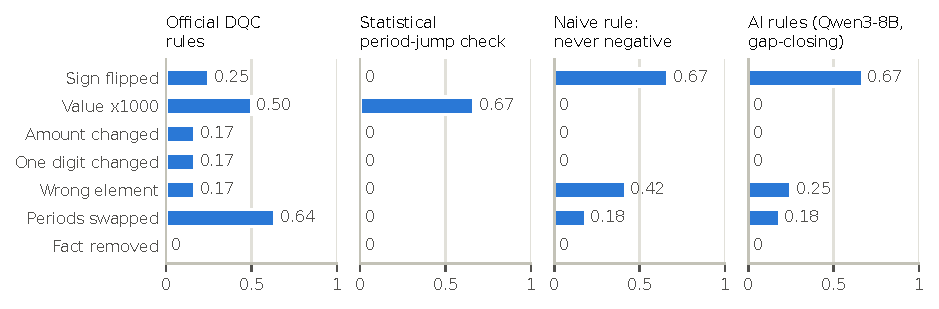
\includegraphics[width=\textwidth]{fig_b_catch.pdf}
\caption{Share of injected errors caught per error type, on the 12 test filings where all controls ran (83 injected errors). ``All existing controls'' combines DQC, the statistical checks and the generic checks.}
\label{fig:catch}
\end{figure}

Added value and alerts (E4 and E5). The best AI rule set added 6 errors beyond the existing controls, but gave on average 458 alerts on a filing that was never corrected (Figure~\ref{fig:alerts}). The statistical checks gave 0.1 to 2.6 alerts and DQC 1.8. None of the nine AI rule sets passed the gate. The alerts came from domain mistakes, not programming mistakes. One rule compared the period type of each fact, stored as ``instant'' or ``duration'', with a list that codes it as ``I'' or ``D'', so it flagged almost every fact. Another assumed that elements with a debit balance can never be negative, which is not true in XBRL \cite{debreceny}. The AI judge caught 2 of 42 injected errors (it could see only 19 of them) and raised about six flags per filing that was never corrected.

\begin{figure}[htbp]
\centering
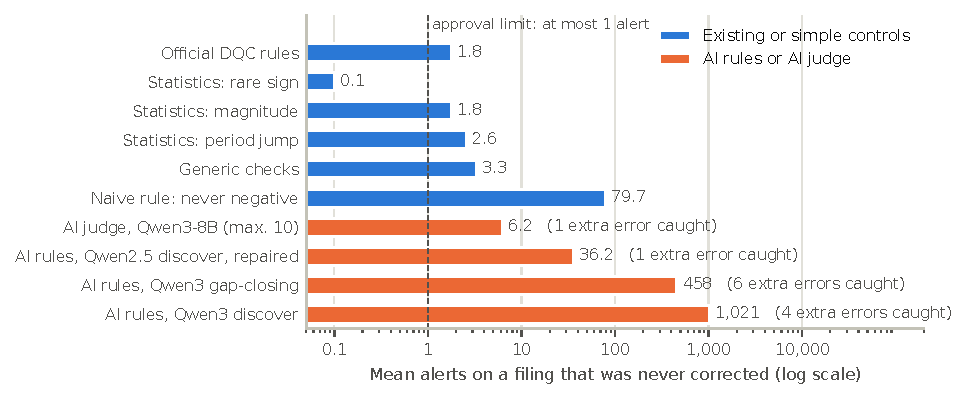
\includegraphics[width=\textwidth]{fig_b_alerts.pdf}
\caption{Mean alerts on test filings that were never corrected (66 filings; DQC on 12; AI judge on 6, at most 10 flags). In brackets: injected errors caught beyond the existing controls. Log scale.}
\label{fig:alerts}
\end{figure}

\section{What this means for the research}

For small local models the pilot gives a clear but preliminary answer. They can sometimes reproduce an expert rule, but not reliably and not stably, and the rules they invent add little beyond the expert rules and statistical checks at a high alert cost. At the same time, the existing controls catch only a third of the injected errors, so there is a real gap that better rules could close. The evaluation design works and measures what a team needs to know. The pilot is small: two small models on a normal processor, DQC on 12 test filings, the judge on 6, stability on nine rules, and no significance tests.

The thesis therefore keeps the design and makes it stronger: larger open-weight models on the GPU cluster, at least three generations per rule, a non-AI rule-suggestion baseline next to the statistical checks, a sample of real corrections checked by a person, the protocol fixed before the final test, and the same design on three to five datasets. It must also handle the domain issues the pilot exposed, such as the meaning of signs and debit or credit balances, values at a moment versus over a period, year-to-date figures, scale, duplicated numbers, company-specific labels and matching the rule version to the taxonomy year. Possible outcomes are that AI rules help only for some error types, or not at all; a clear negative result still tells a team what evidence to ask for before adopting an AI-written rule.

\section{Engineering artefact}

The pilot produced a working command-line tool, \texttt{dqstress}, that follows the steps of a data team onboarding a source. The team registers the source and runs its existing controls, including the statistical checks. The tool then stress-tests these controls with injected errors and reports, per error type, what slips through. A local model can propose rules for those gaps. Each proposal runs in the sandbox, is tested on held-out data and is checked against the gate. A person records the decision, and the tool writes a report with the evidence: which errors the rule catches, how many alerts it gives on clean data, and whether repeated generations agree. For the credit team in the example, ``the AI suggested twenty rules'' becomes a short list of rules with evidence, of which perhaps none or a few are worth adopting. The tool does not change data, does not connect to production systems and never approves a rule by itself.

\begin{thebibliography}{99}
\small
\setlength{\itemsep}{2pt}
\setlength{\parskip}{0pt}

\bibitem{tran} L. Tran, correspondence with the author, 4 September 2026 (unpublished; observations specific to his working context).

\bibitem{alderse} T. Alderse Baas, ``A Real-Life Machine Learning Journey,'' Rabobank Techblog, 15 September 2021. \url{https://rabobank.jobs/en/techblog/a-real-life-machine-learning-journey/}

\bibitem{rehberger} T. Rehberger, T. H\"utter, L. Ehrlinger, and W. W\"o{\ss}, ``Evaluating Data Quality Tools: Measurement Capabilities and LLM Integration,'' arXiv:2604.09163, 2026.

\bibitem{abedjan} Z. Abedjan, X. Chu, D. Deng, R. C. Fernandez, I. F. Ilyas, M. Ouzzani, P. Papotti, and M. Stonebraker, ``Detecting Data Errors: Where are we and what needs to be done?,'' Proceedings of the VLDB Endowment, vol. 9, no. 12, pp. 993--1004, 2016. doi:10.14778/2994509.2994518.

\bibitem{deequ} S. Schelter, D. Lange, P. Schmidt, M. Celikel, F. Biessmann, and A. Grafberger, ``Automating Large-Scale Data Quality Verification,'' Proceedings of the VLDB Endowment, vol. 11, no. 12, pp. 1781--1794, 2018. doi:10.14778/3229863.3229867.

\bibitem{cdc} S. J\"ager and F. Biessmann, ``From Data Imputation to Data Cleaning: Automated Cleaning of Tabular Data Improves Downstream Predictive Performance,'' Proceedings of AISTATS, PMLR 238, pp. 3394--3402, 2024.

\bibitem{raha} M. Mahdavi, Z. Abedjan, R. C. Fernandez, S. Madden, M. Ouzzani, M. Stonebraker, and N. Tang, ``Raha: A Configuration-Free Error Detection System,'' Proceedings of SIGMOD, pp. 865--882, 2019. doi:10.1145/3299869.3324956.

\bibitem{zeroed} W. Ni, K. Zhang, X. Miao, X. Zhao, Y. Wu, Y. Wang, and J. Yin, ``ZeroED: Hybrid Zero-Shot Error Detection Through Large Language Model Reasoning,'' Proceedings of ICDE, pp. 3126--3139, 2025. doi:10.1109/ICDE65448.2025.00234.

\bibitem{autotest} Q. Chen, Y. He, R. C.-W. Wong, W. Cui, S. Ge, H. Zhang, D. Zhang, and S. Chaudhuri, ``Auto-Test: Learning Semantic-Domain Constraints for Unsupervised Error Detection in Tables,'' Proceedings of the ACM on Management of Data, vol. 3, no. 3, 2025. doi:10.1145/3725396.

\bibitem{taberr} P. Jung, S. J\"ager, N. Chandler, and F. Biessmann, ``Towards Realistic Error Models for Tabular Data,'' ACM Journal of Data and Information Quality, vol. 17, no. 4, article 28, 2025. doi:10.1145/3774914.

\bibitem{ledqer} A.-C. Glock, T. H\"utter, J. F\"urnkranz, W. W\"o{\ss}, A. Dominka-Kiss, and L. Ehrlinger, ``Data Quality Rule Generation with LLMs,'' arXiv:2609.06053, 2026.

\bibitem{akella} A. Akella, A. Kaul, K. Narayanam, and S. Mehta, ``Quality Assessment of Tabular Data using Large Language Models and Code Generation,'' Proceedings of EMNLP 2025: Industry Track, pp. 2713--2748, 2025. doi:10.18653/v1/2025.emnlp-industry.183.

\bibitem{audq} J. Biggiogera, N. Colombo, K. Saxena, B. Sarmah, and S. Pasquali, ``AuDQ: Auditable Data Quality through Agentic Rule Discovery,'' arXiv:2610.26031, 2026.

\bibitem{alexander} R. Alexander, L. Katz, C. Moore, M. W.-C. Wong, and Z. Schwartz, ``Evaluating the Decency and Consistency of Data Validation Tests Generated by LLMs,'' arXiv:2310.01402, 2023.

\bibitem{martin} A. Martin, E. C. de Almeida, O. Romero, and A. Queralt, ``How and Why False Denial Constraints are Discovered,'' Proceedings of the VLDB Endowment, vol. 18, no. 10, pp. 3477--3489, 2025. doi:10.14778/3748191.3748209.

\bibitem{ouyang} S. Ouyang, J. M. Zhang, M. Harman, and M. Wang, ``An Empirical Study of the Non-Determinism of ChatGPT in Code Generation,'' ACM Transactions on Software Engineering and Methodology, vol. 34, no. 2, 2025. doi:10.1145/3697010.

\bibitem{homayouni} H. Homayouni, S. Ghosh, and I. Ray, ``An Approach for Testing the Extract-Transform-Load Process in Data Warehouse Systems,'' Proceedings of IDEAS, pp. 236--245, 2018. doi:10.1145/3216122.3216149.

\bibitem{jenga} S. Schelter, T. Rukat, and F. Biessmann, ``JENGA: A Framework to Study the Impact of Data Errors on the Predictions of Machine Learning Models,'' Proceedings of EDBT, pp. 529--534, 2021.

\bibitem{just} R. Just, D. Jalali, L. Inozemtseva, M. D. Ernst, R. Holmes, and G. Fraser, ``Are Mutants a Valid Substitute for Real Faults in Software Testing?,'' Proceedings of FSE, pp. 654--665, 2014. doi:10.1145/2635868.2635929.

\bibitem{secfintables} S. Ke, Q. Wu, H. Li, and L. Cao, ``SEC-FinTables: Evaluating Large Language Models for Detecting Logical Inconsistencies on Tabular Data,'' Findings of ACL 2026, pp. 15587--15607, 2026. doi:10.18653/v1/2026.findings-acl.764.

\bibitem{finauditing} Y. Wang, K. Wang, S. Yang, J. Patel, et al., ``FinAuditing: A Financial Taxonomy-Structured Multi-Document Benchmark for Evaluating LLMs,'' arXiv:2510.08886, 2025.

\bibitem{parasuraman} R. Parasuraman and D. H. Manzey, ``Complacency and Bias in Human Use of Automation: An Attentional Integration,'' Human Factors, vol. 52, no. 3, pp. 381--410, 2010. doi:10.1177/0018720810376055.

\bibitem{shankar} S. Shankar, R. Garcia, J. M. Hellerstein, and A. G. Parameswaran, ``We Have No Idea How Models will Behave in Production until Production: How Engineers Operationalize Machine Learning,'' Proceedings of the ACM on Human-Computer Interaction, vol. 8, no. CSCW1, 2024. doi:10.1145/3653697.

\bibitem{esef} XBRL International, ``filings.xbrl.org,'' public repository of ESEF filings. \url{https://filings.xbrl.org}

\bibitem{debreceny} R. Debreceny, S. Farewell, M. Piechocki, C. Felden, and A. Gr\"aning, ``Does it add up? Early evidence on the data quality of XBRL filings to the SEC,'' Journal of Accounting and Public Policy, vol. 29, no. 3, pp. 296--306, 2010. doi:10.1016/j.jaccpubpol.2010.04.001.

\bibitem{dqc} XBRL US Data Quality Committee, ``DQC rules (dqc\_us\_rules),'' rules, documentation and test suite, version 31, commit 5f8cd32. \url{https://github.com/DataQualityCommittee/dqc_us_rules}; overview at \url{https://xbrl.us/data-quality/rules-guidance/}

\bibitem{arelle} Arelle, open-source XBRL platform, version 2.47.3. \url{https://arelle.org}

\bibitem{brown} N. C. Brown, R. M. Crowley, and W. B. Elliott, ``What Are You Saying? Using Topic to Detect Financial Misreporting,'' Journal of Accounting Research, vol. 58, no. 1, pp. 237--291, 2020. doi:10.1111/1475-679X.12294.

\bibitem{uci-credit} I.-C. Yeh, ``Default of Credit Card Clients,'' UCI Machine Learning Repository, 2009. doi:10.24432/C55S3H.

\bibitem{uci-bank} S. Moro, P. Rita, and P. Cortez, ``Bank Marketing,'' UCI Machine Learning Repository, 2014. doi:10.24432/C5K306.

\bibitem{uci-wine} P. Cortez, A. Cerdeira, F. Almeida, T. Matos, and J. Reis, ``Wine Quality,'' UCI Machine Learning Repository, 2009. doi:10.24432/C56S3T.

\bibitem{fsds} U.S. Securities and Exchange Commission, ``Financial Statement Data Sets,'' quarters 2023q1 to 2025q2. \url{https://www.sec.gov/data-research/sec-markets-data/financial-statement-data-sets}

\bibitem{gleif} Global Legal Entity Identifier Foundation, ``Data Quality Management,'' including the Data Quality Rule Setting. \url{https://www.gleif.org/en/lei-data/gleif-data-quality-management/}

\bibitem{hmda} Federal Financial Institutions Examination Council and Consumer Financial Protection Bureau, ``Filing Instructions Guide for HMDA data collected in 2024.'' \url{https://ffiec.cfpb.gov/documentation/fig/2024/overview}

\bibitem{qwen25coder} B. Hui, J. Yang, Z. Cui, J. Yang, et al., ``Qwen2.5-Coder Technical Report,'' arXiv:2409.12186, 2024.

\bibitem{qwen3} A. Yang, A. Li, B. Yang, B. Zhang, et al., ``Qwen3 Technical Report,'' arXiv:2505.09388, 2025.

\bibitem{gptoss} OpenAI, ``gpt-oss-120b \& gpt-oss-20b Model Card,'' arXiv:2508.10925, 2025.

\bibitem{lucario} Q. Qin, H. Li, and E. Merlo, ``Unsupervised, Robust, and Lightweight Detection of Data Pattern Anomalies and Outliers,'' Information and Software Technology, vol. 192, article 108035, 2026. doi:10.1016/j.infsof.2026.108035.

\bibitem{riolu} Q. Qin, H. Li, E. Merlo, and M. Lamothe, ``Automated, Unsupervised, and Auto-Parameterized Inference of Data Patterns and Anomaly Detection,'' Proceedings of ICSE, pp. 2419--2431, 2025. doi:10.1109/ICSE55347.2025.00078.

\bibitem{rein} M. Abdelaal, C. Hammacher, and H. Schoening, ``REIN: A Comprehensive Benchmark Framework for Data Cleaning Methods in ML Pipelines,'' Proceedings of EDBT, pp. 499--511, 2023. arXiv:2302.04702.

\end{thebibliography}

\end{document}
